\printbibliography[title=참고문헌]

\AppendixTitleToToc
\AttachAppendixTitleToSecnum

\appendix
\appendixpage*

%\chapterstyle{appendixdefault}
%\pagestyle{hangul}

\section{Github Codespace에서 ihaskell-notebook 실행하기}
TODO

\begin{center}
\includegraphics{GithubCodespace0.png}
\end{center}

TODO

\begin{center}
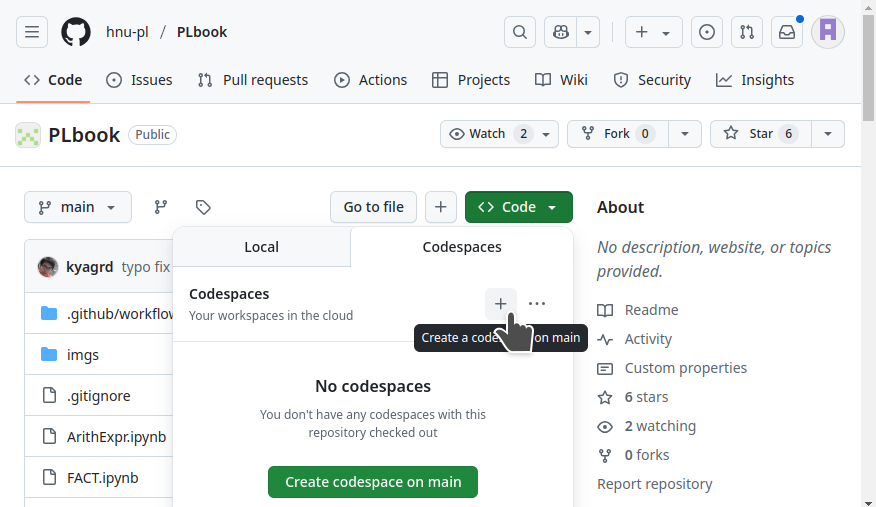
\includegraphics{GithubCodespace1.png}
\end{center}

TODO

\begin{center}
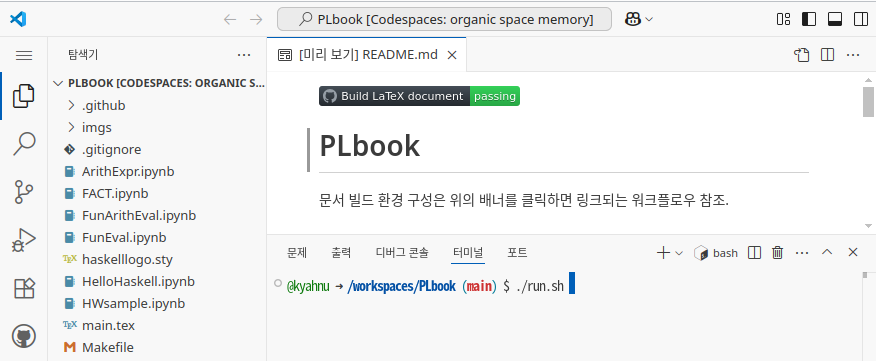
\includegraphics{GithubCodespace2.png}
\end{center}

TODO

\begin{center}
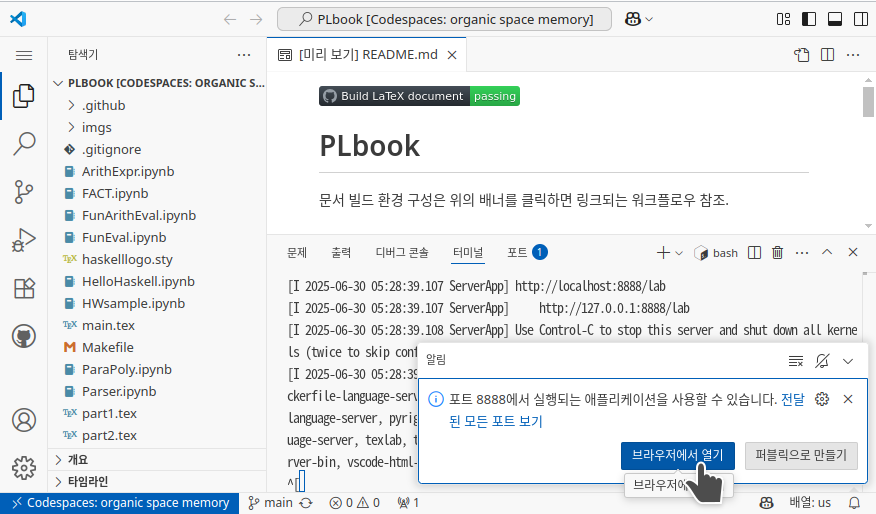
\includegraphics{GithubCodespace3.png}
\end{center}

TODO

\begin{center}
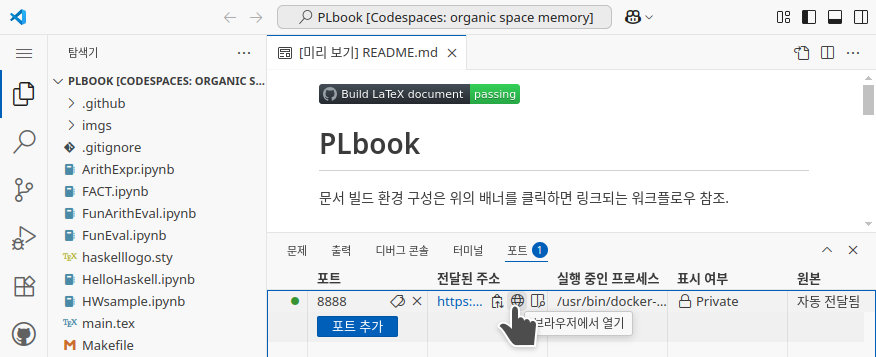
\includegraphics{GithubCodespace4.png}
\end{center}

TODO

\newpage

\section{과제 형식 예시}
\input{HWsample}

\newpage

\section{감사}
강의 노트를 교재의 형태로 이렇게 출간할 수 있게 된 데는 제가 컴퓨터과학을 전공하면서
인연을 맺게 된 은사님들과 정보과학회 프로그래밍언어연구회의 모든 분들에게 마땅히 감사한 마음이 있습니다.
하지만 여기에서 감사의 말씀을 표하기에는 너무 길어지는 관계로,
우선 이 책의 출간 과정에 직접적인 도움을 주신 출판사 관계자 분들,
수업 중에 오탈자를 보고해 준 수강생들, 그리고 프로그래밍언어론 과목에서
대학원생 조교로 수업 운영을 도우며 출판사를 섭외하는 등 다방면으로
신경써 준 제자인 손범준에게 이 지면을 빌어 간단히나마 감사의 기록을 남깁니다.

\subsection{초판 원고 작업본 오탈자 보고}
\subsubsection{2022년 1학기 프로그래밍언어론 수강생}
구준한, 권준호, 권혁준, 김동하, 김상운, 김이레, 김현, 백성욱, 백창현, 손현승,
신현수, 이승민, 이상빈, 장주안, 임영준, 장태영, 전석원, 정윤정, 정재훈, 황인규.

\subsubsection{2023년 1학기 프로그래밍언어론 수강생}
김민식, 김종윤, 박준형, 서지웅, 신수민, 윤승준, 이동복, 이재혁, 임도은, 정종운.

\subsubsection{2024년 1학기 프로그래밍언어론 수강생}
김지민, 문해찬, 명현철, 성재빈, 성준모, 장민혁, 유진호, 이강준, 이규호, 이승현, 이정아, 최태규, 한성준.

\begin{comment}
\newpage

\section{다음 판에 추가할지 고려중인 주제}
\subsection{Control}
Continuation-Passing Style,
Delimited Continuations,
Coroutines, Exceptions, Async-Await,
Algebraic Effects,
Functor/Applicative/Monad/Monoid/...

\url{https://www.microsoft.com/en-us/research/wp-content/uploads/2016/08/algeff-tr-2016-v2.pdf}

\subsection{Staged Computation}
Interpreter vs. Compiler, Futamura Projections, Partial Evaluation

\end{comment}


